\chapter{Literature Review} \label {ch:theory}
%Write about the theory used in the research.
\emph{The chapter gives both general and specific information on theory used for this project.  Mathematical statistics, regression and machine learning are covered in the first three sections, providing a general understanding of the field of study. Specific machine learning models are explained in the final three sections of the chapter. }


\section{Supervised learning} \label{sec:supervisedlearning}
	In supervised learning, the learner (algorithm) receives a dataset of labeled observations which is used to predict correct values for unseen data\cite{BOOK:3}. A database table storing weather-related data could for example have thousands of records (observations) where data in each record belong to certain columns (features) such as wind speed $w_s$, wind direction $w_d$ and time $t$. The goal of supervised learning is to build a mathematical model
\begin{equation} \label{eq:mappingfunction}
	y = f_{map}(x)
\end{equation}
such that when new input data is used, $f_{map}$ is able to predict a correct output value \cite{WEBSITE:3}. The model is built from a dataset which is typically split into three parts \cite{WEBSITE:4}:

\begin{itemize}
	\item {Training dataset:} Used to fit the model.
	\item {Validation dataset:} Used to give an unbiased evaluation of a model built from the training dataset and potentially update its hyperparameters. Hyperparameters are model parameters that are used in some learning algorithms. They are usually fixed before the training process begins \cite{WEBSITE:7}.
	\item {Test dataset:} Gives an unbiased evaluation of the final model.
\end{itemize}
	How the dataset "should" be split is brought up in section \ref{sec:datasetsplit}. 

	Supervised learning can be thought of as having a teacher supervising the algorithm. The correct answers are in the training data and the algorithm learns from being corrected by the teacher \cite{WEBSITE:3}. Going back to the forementioned example of the weather station to give a brief example of how a supervised machine learning algorithm works: Suppose a training, validation and test dataset is provided and one wishes to predict wind speed $y = w_s$ based on wind direction and time $x = [x_1, x_2] = [w_d, t]$. During the training process, a supervised learning algorithm goes through the training dataset to build a model, as seen in Eq. \ref{eq:mappingfunction}, and possibly updated when validated against the validation dataset. Suppose the supervised learning algorithm used is multiple linear regression (see section \ref{sec:reg_based_learning}) and a model is built from the training process: 

\begin{equation} \label{eq:example_ws}
	w_s = f_{map}([w_d, t]) = \beta_0 + \beta_1 w_d + \beta_2 t = 4 + 0.2w_d + 1.7t
\end{equation}
	The model can then be tested with the test dataset to see how it performs on unseen data. 

	Estimation of continous output variables, such as wind speed in the example presented above, is a regression problem. In supervised learning there are also algorithms associated with the problem of classification; how to categorize data \cite{WEBSITE:8}.


	\subsection{Classification predictive modeling} \label{sec:classification}
	In a classification problem, the computer is asked to place a new observation into one of $k$ categories (labels), $k \geq 2$ \cite{BOOK:1}. The problem of categorizing new email as spam or not spam is an example of a classification problem. Google claims that their machine learning models can detect spam and phishing messages with 99.9\% accuracy in their widely used Gmail application \cite{WEBSITE:4}. Classification on two labels, as in the forementioned example, is known as a binary classification case and problems with three or more labels to be classified is called multiclass classification case \cite{MISC:1}. Classifying precipation type is a multiclass classification case since it has more than two labels.

	Another example of a classification problem, one that may well be the first that machine learning novices encounter, is classification of the Iris flower dataset. The dataset consists of 50 observations with four features: length and width of the sepals and petals, in centimeters. Based on this information, the problem is to classify to which of the following labels each observation belongs to \cite{WEBSITE:5}:

\begin{itemize}
	\item Setosa
	\item Versicolour
	\item Virginica
\end{itemize}

	How the classification is carried out depends on the algorithm used to build the model. These kind of algorithms are commonly known as classifiers. There are several classifiers that can be used for the Iris dataset, but their performance in doing so may differ. Performance of classifiers are typically measured in accuracy, which is the amount of correct predictions divided by the number of observations in the test dataset \cite{BOOK:1}.
%ta upp vilka performance measures är bäst

\begin{equation}
	\mbox{accuracy} = \frac{\mbox{\#correct predictions}}{\mbox{\#observations}}
\end{equation}
	
	\subsection{Regression predictive modeling} \label{sec:regression}
	In contrast to classification problems, such as categorizing incoming email as spam or not spam, regression problems are about predicting continous quantaties. Regression models can have either real-valued or discrete input variables. The model in eq. \ref{eq:example_ws} is an example of a regression model since the goal is to predict a numerical value for wind speed. The problem could be translated into a classification problem by, for example stating that for given numerical intervals, the wind speed is categorized as being low, medium or high. This kind of conversion is known as discretization. But even if the conversion is useful, it can result in surprising and/or poor performance \cite{WEBSITE:8}. This is why both classification and regression modeling are covered in this project because one is used to classify, the other is used to predict.

%ta upp vilka performance measures är bäst
	Performance of regression models can be measured by computing the mean squared error (MSE) of the model on the test dataset. 
\begin{equation}
	MSE_{test} = \frac{1}{n} \sum_{i}^{n}(y'_{test} - y_{test})_{i}^2
\end{equation}
where $y'_{test_i}$ are predictions on the test and $y_{test_i}$ are actual values \cite{BOOK:1}. It's a measurement of how close each prediction was to its corresponding target value on average.

\section{Generalization}
	During the training process in supervised learning, a model is typically built based on its training data, and updated in order to reduce its training error. But the fundamental goal of machine learning is to generalize beyond observations in the training dataset since it's unlikely that the same exact observations are found again on unseen data \cite{ARTICLE:3}. This is why test datasets are used to measure performance of regression and classification models as seen in sections \ref{sec:regression} and \ref{sec:classification}. Both training error, how well a performs on its training data, and generalization error, how well a model performs on unseen data, need to be considered in machine learning \cite{BOOK:1}.

	The terminology used to explain how well machine learning models learn and generalizes to new data is overfitting and underfitting \cite{WEBSITE:8} which are two central challenges in machine learning \cite{BOOK:1}. 
\begin{itemize}
	\item{Overfitting:} Random fluctuations and statisticical noise is learnt to the extent that it affects the model's ability to generalize \cite{WEBSITE:8}. Instead of learning the data trend in the training data, the model "memorizes" it \cite{ARTICLE:4}. Non-linear (see section \ref{}) and non-parametric (see section \ref{}) models are prone to overfitting as they are flexible in choosing mathematical functions to fit its training data \cite{WEBSITE:8}.  
	\item{Underfitting:} A model that performs poorly on both its training data and on generalization. If a good performance metric is used, underfitting is  easy to detect \cite{WEBSITE:8}.
\end{itemize}
The goal then, is to select a model that is somewhere between underfitting and overfitting. Underfitting is typically remedied by choosing alternative models, but the most common problem in applied machine learning is how to avoid overfitting \cite{WEBSITE:8}. According to Davide \cite{ARTICLE:4}  the mere awareness of the issue of overfitting along with two powerful tools: cross-validation and regularization, can be enough to overcome the problem.

	\subsection{Cross-validation}
	There are several cross-validation techniques out of which the most commonly used is k-fold cross validation: Once a randomly shuffled dataset is split into a training and test dataset, the training dataset is further split into $k$ folds. One fold is used as a validation dataset and the remainding for training. The idea is to iterate this process $k$ times so that every fold has been used once as a validation set, and ultimately average the performance over $k$ iterations . Using a value of $k = 10$ is a common choice in practice and in which case it is called 10-fold cross-validation \cite{ARTICLE:4}. Furthermore, using $k=10$ seems to be optimal when it comes to optimizing run-time for the test, limiting bias (underfitting) and variance (overfitting) \cite{BOOK:4}.   

	There is a variant of this technique called stratified k-fold cross-validation which is mostly used in classification problems.  In stratified k-fold cross-validation the folds are created in such a way that each fold contains similar proportions of predictor labels as the full dataset. For example, think of the classification problem of classifying email as spam or not spam. If the ratio of spam/not spam is 20\%/80\% in the original dataset, then the same proportion is attempted to be maintained in each of the $k$ folds. This technique tends to generate less bias and variance when compared to regular k-fold cross validation \cite{IP:2}. It can also be applied to regression problems \cite{WEBSITE:10} but the results from Breiman and Spector \cite{ARTICLE:5} indicate that there is little improvement from using this technique for regression problems.

	\subsection{Regularization} \label{sec:regularization}
	The second method of overcoming overfitting is regularization. This technique discourages complexity and flexibility of models by regularizing its coefficients toward zero \cite{WEBSITE:13}. The magnitude of the regularization can be controlled by a hyperparameter $\lambda$ \cite{WEBSITE:12}. The higher value of $\lambda$, the higher impact regularization has on the model, but high values on $\lambda$ can result in underfitting and should therefore be controlled carefully \cite{WEBSITE:13}. Three different types of regularization methods as covered by \cite{WEBSITE:12}:

\begin{itemize}
	\item{$L_1$ regularization (Lasso):} Adds a penalty equal to the sum of the absolute values of $n$ coefficients. This kind of regularization can nullify parameters and for that reason it can be seen as a way to limit the amount of features in the model (see \ref{sec:feature_selection}).
		\begin{equation}
			Error_{L_1} = Error + \lambda \sum_{i=1}^{n}|\beta_i| 
		\end{equation}
	\item{$L_2$ regularization (Ridge):} Adds a penalty equal to the sum of the square value of the coefficients. This exhibits a different behavior than $L_1$ regularization in that the coefficients are slowly reduced to zero.
		\begin{equation}
			Error_{L_2} = Error + \lambda \sum_{i=1}^{n}\beta_i^2 
		\end{equation}
	\item{$L_1/L_2$ regularization (Elastic-net):} A combination of $L_1$ and $L_2$ regularization. Here, a value $\alpha$ is set to determine the impact ratio of $L_1$ and $L_2$ regularization, where $0 \leq \alpha \leq 1$.
 		\begin{equation}
			Error_{L_1L_2} = Error + \lambda ( (1-\alpha)\sum_{i=1}^{n}|\beta_i| + \alpha  \sum_{i=1}^{n}\beta_i^2 ) 
		\end{equation}
\end{itemize}
%Regularization can be used in any parametric (see section \ref{}) machine learning algorithm \cite{WEBSITE:11}.

	\subsection{Feature selection} \label{sec:feature_selection}
		Feature selection is a process where irrelevant and redundant features are removed. The curse of dimensionality, which is brought up in \ref{sec:background}, can be avoided by reducing the amount of features. Fewer features can also make the model more interpretable and shorten the training time. Furthermore, reducing the dimensionality results in better generalization \cite{ARTICLE:10}.  
	
	%Reduced dimensionality gives better generalization due to fewer model parameters in the data \cite{ARTICLE:10} 

%"Feature subset selection is the process of identifying and removing as many irrelevant and redundant features as possible. This reduces the dimensionality of the data and enables data mining algorithms to operate faster and more effectively. The fact that many features depend on one another often unduly influences the accurary of supervised ML classification models. this problem can be addressed by constructing new features from the basic feature set." \cite{ARTICLE:7}

% Multicollinearity
%"When you add more input variables it creates relationships among them. So not only are the input variables potentially related to the output variable, they are also potentially related to each other, this is referred to as multicollinearity. The optimal scenario is for all of the input variables to be correlated with the output variable, but not with each other." https://medium.com/@MaximilianLloyd/multiple-linear-regression-in-machine-learning-4711209604b7 

%http://scikit-learn.org/stable/modules/feature_selection.html
	\begin{itemize}
		\item{Filter method:}
		\item{Wrapper method:}
		\item{Embedded method:}
	\end{itemize}
	
\section{Supervised learning algorithms} \label{sec:supervised_algorithms}
	There are many algorithms that can be used to solve regression and classification problems, some of which can solve both. There is a famous theorem called the "no free lunch" theorem which contradicts an ideal case where a single machine learning is best at solving all possible machine learning problems \cite{ARTICLE:5}.  It is therefore interesting to study the effect of different supervised learning algorithms in this project, but to explain the functionality of them in detail is out of scope. Instead, the reader is encouraged to look up details on specific algorithms elsewhere. The algorithms are grouped by similarity in this section, which is referred to as algorithm families. The algorithm families are named the same way as in \cite{BOOK:6}. Each family listed in \ref{sec:delimitations} are covered. 

	\subsection{Decision tree based learning}
		Decision tree algorithms uses a decision tree datastructure to solve classification and regression problems. Furthermore, Non-leaf nodes represent conditions for a specific feature and leaves are values of the target feature. One of the main advantages of decision tree algorithms is that they are easy to understand \cite{ARTICLE:7}. Figure \ref{fig:decisiontree_example} depicts an example of a decision tree used to solve a classification problem with two features: sex and age. Starting at the root node, a decision is made once a leaf-node is reached. Ideally, the feature that best divides the dataset would be represented in the root of the tree, followed by the second best in the second level etc. However, constructing such optimal decision trees has been proved to be a NP-complete problem \cite{ARTICLE:11}. 

\begin{figure}[H] 
	\centering
	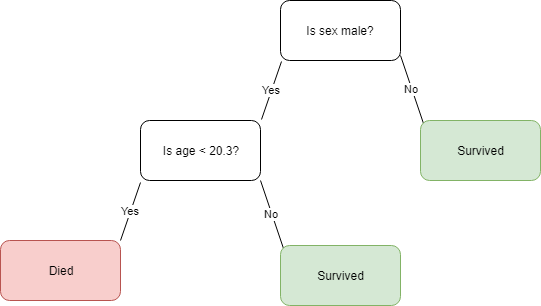
\includegraphics[width=0.8\textwidth]{media/decisiontree_example.png}
	\caption{Example of a decision tree which predicts if a passenger survives a car crash or not.}
	\label{fig:decisiontree_example}
\end{figure}

		Decision tree algorithms are allowed to capture non-linear patterns in the training data, which makes them flexible, but also prone to overfitting \cite{BOOK:7}. Kotiantis \cite{ARTICLE:7} claims there are two common solutions to battle overfitting in decision tree induction algorithms:
		\begin{enumerate}
			\item Stop the training before it fits the training data perfectly
			\item Prune the decision tree
		\end{enumerate}
		The second method has shown to be more successful in practice than the first one \cite{BOOK:8}. Pruning is a process in which subtrees of the decision tree are replaced by leaves. In other words, the size of the tree is reduced. There are different pruning methods that can be used, but exploring such details are not in the scope of this project.

		 Among several decision tree induction algorithms, CART and C4.5 are the most commonly used \cite{BOOK:8}. CART can solve both regression and classification problems and it is available in Scikit-learn \cite{WEBSITE:16}. %CART can be used to solve multiclass classification problems \cite{ARTICLE:16}
		
	\subsection{Instance based learning}
	Instance-based learning (IBL) is about storing the provided training data, and using it to predict/classify a new observation. In other words, when a new observation is received, an IBL algorithm retrieves related observations from memory and uses it to predict/classify the new observation. This behavior means that IBL algorithms process training data quickly while the classification/prediction process takes more time when compared to, for example, decision trees \cite{ARTICLE:8}. 

	An example of an IBL algorithm is $k$-nearest neighbor (kNN). Generally, observations can be considered to be points in an $n$-dimensional space and kNN is based on the principle that these observations in a dataset are generally close to other observations with similar properties.  For a new observation, the algorithm finds the $k$ closest neighbors and uses the properties of the $k$ neighbors to classify the observation. kNN can be used to solve both regression and multiclass classification problems in Scikit-learn \cite{WEBSITE:17, WEBSITE:18}.

	Wu et. al \cite{ARTICLE:9} argue that kNN is suitable for multiclass classification problems. Another study by L. Zhong et. al \cite{IP:3} showed success in predicting CT images from MRI data by using kNN regression. However, \cite{ARTICLE:9} mentions that the algorithm is sensitive to the choice of $k$: smaller values can mean it is sensitive to noise and larger values may include too many points from other classes. Overall, Okamoto and Yugami \cite{ARTICLE:12} showed that an optimal choice of $k$ grew linearly with an increase in the amount of training instances. This indicates that $k$ should be higher for higher amount of training data. However, scientific methods for choosing a specific optimal value of $k$  are lacking \cite{ARTICLE:7}.

	Wu et. al \cite{ARTICLE:9} talks about the issues of choosing a distance metric for kNN. They say that among several choices, it is desirable to have a distance measure in which a smaller value between two nodes implies a stronger connection. Scaling is another issue they talk about when it comes to distance metrics. If one feature $f_1$ varies from, say 1.5 to 1.8, and another $f_2$ from 10,000 to 1,000,000 then $f_2$ will have higher impact on the computation of distance. 
	
	%\subsection{Kernel methods based learning}
	
	\subsection{Bayesian learning}
		Bayesian algorithms are those that apply the Bayesian inference theorem. This can be used to calculate the probability of a hypothesis $H$ after seeing the data $D$.
		\begin{equation} \label{eq:bayes}
			p(H|D) = \frac{p(H)p(D|H)}{p(D)}
		\end{equation} 
	The basic notion of this kind of algorithms is that classification can be achieved if assumptions can be made from existing data. %Imagine an example of seeing a person whose sex you cannot decide, and you wish to address this person from afar. The person is standing in queue for the men's room, would you call out "excuse me ma'am" or "excuse me sir"? One may assume that this is a man since there is a higher probability of men being in line for the men's room than vice versa. 

	Naïve Bayes classifiers assume that the features in a dataset are independent from one another. Which means that each feature contribute independently to classify an observation, regardless of any correlations that might exist among the features, which is why it is called naïve. Despite this naïve assumption and its ease of use, Naïve Bayes classifiers have proved successful, even when strong dependencies among features are present \cite{ARTICLE:13, IP:4}. Naïve Bayes can be applied to regression problems through discretization, but it has limited success in comparison to classification problems when the independence assumption does not hold \cite{ARTICLE:14}. Naïve Bayes can be applied to multiclass classification problems \cite{ARTICLE:17}. 

	The Gaussian Naiïve Bayes classifier assumes that the features have a gaussian (normal) data distribution.
	 
	\subsection{Regression based learning} \label{sec:reg_based_learning}
		As stated in \ref{sec:delimitations}, only linear algorithms of Regression based learning agorithms are covered. A linear algorithm is one where its model is specified as a linear combination of input features.  

		Although the names might be confusing, regression based learning is not the same as regression predictive modelling, which are referred to as "regression problems" throughout this project. Regression based analysis refers to regression analysis: a number of statistical methods for estimating relationships among variables. This is a well-known tool in statistics and it is also used in machine learning. 

		There are three components in a regression model: scalars $\beta_i$, independent variables $X_i$ and dependent variables $Y$. In regression based learning, $X_i$ represent input features, $Y$ is the target feature and $\beta_i$ are parameters which are tuned during the training process. The example shown in \ref{eq:example_ws} is an example of a trained regression based learning algorithm called Ordinary Least Squares (OLS). OLS is used in regression predictive modelling and a different regression based learning algorithm called Logistic regression (LR) can be used for classification problems. 

		Some of the assumptions listed by \cite{BOOK:6} that most regression based learning algorithms make of the training data:
	\begin{itemize}
		\item{Linear behavior:} If a target feature and an input feature have a linear relationship, it would look like a straight line when plotted against oneanother. Any non-linear dependencies between the target feature and other features are assumed to not be considered input features.
		\item{Normal distribution:} Assumes the data of the target feature is normally distributed.
		\item{Outliers:} Are expected to be handled.
		\item{Data accuracy:} Values of the target feature that are consider for classification/prediction are assumed to be deleted. For example, error states that are not to be classified.
	\end{itemize} %skriv mer om assumptions?

		In addition to applying cross-validation, overfitting in regression based learning algorithms can be thwarted by applying the regularization techniques as seen in \ref{sec:regularization}. Feng et. al \cite{ARTICLE:15} chose $\lambda$, which is one of the regularization hyperparameters,  based on which value of $\lambda$ maximised their cross-validation scores. They did so by performing a grid-search (see \ref{sec:hyperparameters}) on $\lambda$. %ex: lambda = e^(x/10), x = -100, -99,...9, 10).http://eds.b.ebscohost.com.proxy.lib.ltu.se/eds/pdfviewer/pdfviewer?vid=6&sid=e3b5f9cf-09c2-4142-81c9-bbfa4b659571@sessionmgr4008

	\subsection{Deep learning}
			Deep learning algorithms are those that aim to learn an artificial neural network (ANN) \cite{BOOK:6}. ANNs take inspiration from biological neural networks found in the human brain. An ANN is a directed weighted graph where each node represents an artificial neuron. The graph is organized from left to right by having three type of nodes:
	\begin{itemize}
		\item Input nodes
		\item Hidden layer nodes
		\item Output nodes
	\end{itemize}
			The input nodes are the different input features and the output nodes are possible outcomes. Without going into too much detail, the hidden layers are there to transform the input to an output. For example, imagine a neural network model trained to recognize triangles. The input nodes represent all of the different pixels. The first hidden layer of that model distinguishes edges in the picture, the second layer recognizes when these edges form complex shapes, and so on. Figure \ref{fig:neuralnetwork_example} depicts an example of a deep learning algorithm model with the same kind of problem as seen in \ref{fig:decisiontree_example}.

\begin{figure}[H] 
	\centering
	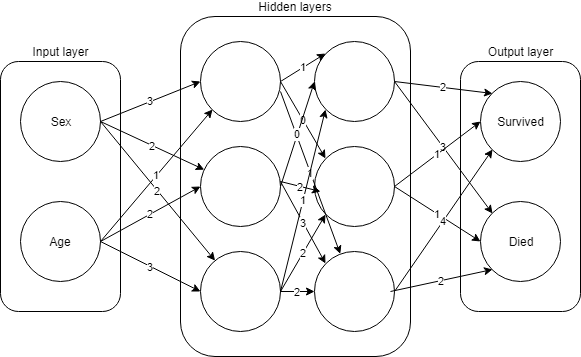
\includegraphics[width=0.8\textwidth]{media/neuralnetwork_ex.png}
	\caption{Example of a neural network with two hidden layers. The goal is to predict if a passenger survives a car crash or not.}
	\label{fig:neuralnetwork_example}
\end{figure}

			The number of hidden layers $h$ and the number of nodes per hidden layer $N_h$ can be configured as hyperparameters in the different deep learning methods. So the question is, what is the optimal value of $h$ and $N_h$? Heaton \cite{BOOK:10} writes that for most practical problems, having $h=1$ is enough for most practical problems and that there is no theoretical reason to use more than two hidden layers. As for $N_h$, Heaton writes that a low value of $N_h$ can lead to underfitting and the opposite may introduce overfitting and a significant increase in training time. The author encourages practitioners to try different values for $N_h$ but provides several rule-of-thumb methods for simplicity, one of which is the following: "The number of hidden neurons should be 2/3 the size of the input layer, plus the size of the output layer". %"The Presence of irrelevant features can make neural network training very inefficient, even impractical" \cite{ARTICLE:7}

			All that's been covered so far of ANNs is the structure, but how are decisions made? Choices are made in the ANN by having each non-input node $n_i$ process information from the previous node whose edge to $n_i$ have the highest value among all nodes connected to $n_i$. In other words, which of the connected nodes to $n_i$ to choose depends on the weights of the edges that connects them. How the weights are set correlates to the learning process, which is what distinguishes the different types of deep learning algorithms.

			Backpropagation is a deep learning algorithm that can be used to solve supervised learning problems. Broadly speaking, backpropagation updates the weights of the edges in the ANN based on a loss function. Whenever a "bad" classification/prediction is made (based on the loss function), the information is propagated backwards in the network from that classification/prediction and weights are adjusted accordingly.

	\subsection{Ensemble learning}
		Ensemble learning is based on the principle that combining the results of several classifiers/predictors into a collective score can produce better results than individual scores. Two independent studies indicate that Random forest, an ensemble learning algorithm, show high success when compared to non-ensemble algorithms\cite{ARTICLE:16, IP:5}. %Chowdhury et. al \cite{ARTICLE:16} conducted a study to see if ensemble methods were superior to CART, kNN, support vector machine and neural network in classifying physical activities. One of the ensemble methods used in the study was Random forest, which showed a constistent high score. Random forest performed second best in an empirical comparison of ten supervised learning algorithms \cite{IP:5}.
		Random forest averages the results from several decision tree classifiers/predictors to achieve a result. Random forest can be applied to classification and regression problems \cite{WEBSITE:17}.

\section{Choosing hyperparameter values} \label{sec:hyperparameters}
	Generally speaking, finding optimal hyperparameter values for various algorithms can be regarded as an experimental process. One brute-force approach, which according to \cite{BOOK:9} is the best way to verify optimality of hyperparameters, is to use a technique known as grid-search. The technique systematically tests hyperparameters incrementally in a given interval. Although the technique may prove useful, it can be computationally intense.
	%The best way to verify hyperparameters for an algorithm applied to specific data is to test them all by cross-validation, and to pick the best combination. This simple approach, called grid-search, offers indisputable advantages by allowing you to sample the range of possible values to input into the algorithm systematically and to spot when the thengeral minimum happens. On the other hand, grid-search has two disadvantages:
	%computationally intense
	% systematic and intensive tests enhance possibility of incurring error because some good but fake validation results can be caused by noise present in the dataset. \cite{BOOK:9}


\section{Dataset split} \label{sec:datasetsplit}
	%https://machinelearningmastery.com/difference-test-validation-datasets/ ( Max Kuhn and Kjell Johnson, Page 78, Applied Predictive Modeling, 2013)

	% why not single testset:
	%– A test set is a single evaluation of the model and has limited ability to characterize the uncertainty in the results.
	%– Proportionally large test sets divide the data in a way that increases bias in the performance estimates.	
	%– With small sample sizes:
	%– The model may need every possible data point to adequately determine model values.
	%– The uncertainty of the test set can be considerably large to the point where different test sets may produce very different results.
	%– Resampling methods can produce reasonable predictions of how well the model will perform on future samples


	
\section{Data preparation}
	\subsection{Imbalanced data}
% {ARTICLE:4} https://www.ncbi.nlm.nih.gov/pmc/articles/PMC5721660/
% tip 5
	%https://machinelearningmastery.com/how-to-prepare-data-for-machine-learning/

	%method to filter out noise, outliers http://ieeexplore.ieee.org/stamp/stamp.jsp?tp=&arnumber=6033571


